%===============================================================================
% ifacconf.tex 2022-02-11 jpuente  
% 2022-11-11 jpuente change length of abstract
% Template for IFAC meeting papers
% Copyright (c) 2022 International Federation of Automatic Control
%===============================================================================
\documentclass{ifacconf}

\usepackage{hyperref}
\usepackage{graphicx}      % include this line if your document contains figures
\graphicspath{ {./images/} }
\usepackage{caption}
\usepackage{natbib}        % required for bibliography
\usepackage{glossaries}    % required for glossary

\makeglossaries
\loadglsentries{glossary}  % loading the glossary.tex file

%===============================================================================
\begin{document}
	
	\begin{frontmatter}
		
		\title{Methods of Reducing Computational Requirements for Large Language Models} 
		% Title, preferably not more than 10 words.
		
		\author[First]{Oleksandr Kononov} 
		
		\address[First]{South East Technological University, 
			Cork Road, Waterford, Ireland (e-mail: 20071032@mail.wit.ie).}
		\begin{abstract}                % Abstract of 50--100 words
			TODO
		\end{abstract}
		
		\begin{keyword}
			Artificial intelligence, Neural networks, 
		\end{keyword}
		
	\end{frontmatter}
	%===============================================================================
	\section{Introduction}
	\subsection{Background}
	A \gls{llm} is neural network model which is capable at working with natural language tasks such as text generation, tmeasurmentext summarization, translation, and more. The novel Transformer architecture proposed in the "Attention Is All You Need" paper \cite{vaswani2017attentionneed} has revolutionized the field by introducing more efficient multi-headed self-attention mechanism compared to Recurrent Neural Networks that came before. With the improvements in training times, better parallelization on GPUs and overall quality of output.
	Following this, OpenAI have used this novel Transformer architecture to design and develop their \gls{gpt} \glspl{llm} the following years. In particular, the release of GPT-3 in 2020, has sparked a global interest in the continued development of \glspl{llm} from various companies such as Meta with LLaMa, Google with Gemma, Antropic with Claude, etc.
	
	The AI researchers at Meta have developed a series of open-weight \glspl{llm} called LLaMa, ranging from 7B parameters to 65B parameters \cite{touvron2023llamaopenefficientfoundation}. Their paper demonstrates, using various benchmark tests, we can draw a correlation between the increase in \glspl{llm} parameters and the scores that it can achieve on various benchmark tests such as HellaSwag \cite{zellers2019hellaswagmachinereallyfinish}, WinoGrande \cite{sakaguchi2019winograndeadversarialwinogradschema}, ARC \cite{clark2018thinksolvedquestionanswering} and OpenBookQA \cite{mihaylov2018suitarmorconductelectricity}. There are challenges with regards to the computational requirements necessary for inferencing \glspl{llm},``the compute and memory requirements of state-of-the-art language models have grown by three orders of magnitude in the last three years, and are projected to continue growing far faster than hardware capabilities" \cite[p.~97]{bommasani2022opportunitiesrisksfoundationmodels}.
	
	Quantization and pruning are some of the strategies that can be used to help reduce computational requirement and memory footprint of \glspl{llm}. However applying these strategies often comes at the cost of increasing the \gls{llm} \gls{ppl}, a metric for evaluation the uncertainty of a model in predicting a sequence. Quantization methods involve reducing the numerical precision of the model's weights, allowing 32-bit floating point value to be represented as an 8-bit floating point value or even lower. Popular quantization include \gls{gguf}\cite{llamacpp, ggml}, \gls{awq}\cite{lin2024awqactivationawareweightquantization}, \gls{vptq}\cite{liu2024vptqextremelowbitvector} and others. Pruning involves removing parts of the model that have little effect on the output, this process could involve removing neurons or entire layers.
	
	\subsection{Problem Statement and Motivation}
	
	As mentioned in the previous section, the hardware requirements for medium to large sized  \glspl{llm} make it difficult for consumers or small organisations to run their own local  \glspl{llm}, often requiring to use third-party providers for access to modern powerful  \glspl{llm}. This potentially reduces their privacy, security and accessibility, which could be otherwise achieved by running  \glspl{llm} locally on their own hardware. For large businesses who might already be hosting their own models, this could be an opportunity to potentially reduce their running costs with regards to \glspl{llm}.
	
	If in the future, smaller \glspl{llm} become more capable than they are today, it stands to reason that their larger counterparts would likewise become more capable. Therefore, finding efficient and cost effective methods of reducing hardware requirements for running large \glspl{llm} is holds meaningful significance to this researcher.
	
	\subsection{Research Scope and Limitations}
	This research will be using a select few foundational \glspl{llm} for testing and evaluation. The selected \glspl{llm} will be Gemma2 9B from Google\cite{gemmateam2024gemma2improvingopen}, LLaMa 3.1 from Meta 8B \cite{dubey2024llama3herdmodels} and Qwen2.5 7B from Alibaba\cite{qwen2.5}. These models were selected due to their research permissive licenses, \gls{llm} community popularity and reputability of the companies that have trained them.
	
	The hardware for conducting this research will be limited to a single Nvidia RTX 4090 GPU with 24GB of VRAM, which will be sufficient to run the selected \glspl{llm} without any quantization. This will allow the researcher to establish baseline metrics and benchmark scores pre-quantization, which can be used to compare against post-quantized results of the selected \glspl{llm}.
	
	The hardware used to demonstrate the effects and performance of \gls{llm} quantization will be a single Raspberry Pi 4b, which has quad-core Cortex-A72 @ 1.5GHz CPU and 8GB LPDDR4 RAM \cite{raspberrypi4}. This device was chosen for it's limited hardware specifications, that should under normal circumstances be insufficient run any of the selected \glspl{llm} previously mentioned. As such, it qualifies to be a test device for this papers research and would serve as a baseline for future research evaluating more capable devices.
	
	This research will be limited to exploring \gls{ptq} methods and not \gls{qat} methods, as the later requires significant computational resources and time in order to carry out such research. \gls{ptq} methods are significantly less computationally intensive to perform on pre-trained \glspl{llm} and require less time to quantize \gls{llm} weights.
	
	\subsection{Research Questions}
	This paper aims to answer the following Research Questions (RQ):
	
	\textbf{RQ1}: What quantization methods (\gls{gguf}, \gls{awq}, \gls{vptq}) are the most effective for reducing selected \glspl{llm} inferencing requirements while retaining most of it's output quality?
	
	\textbf{RQ2}: What pruning strategies (block-wise, channel-wise, layer-wise) are the most effective for reducing selected \glspl{llm} inferencing requirements while retaining most of it's output quality?
	
	\textbf{RQ3}: Deriving the best performing method (or combination of methods) from the previous questions, what is the best achievable performance of selected \glspl{llm} on a Raspberry Pi 4b?
	
	
	\section{Preliminary Literature Review}
	This section will explore the supporting research literature that will cover the topics of various \gls{ptq} methods, pruning methods and what kind of benchmark tests exist for \gls{llm} evaluation that are used in the industry. 
	
	\subsection{\gls{llm} \gls{ptq} Methods}
	Arguably, one of the most well known \gls{llm} quantization method within the open-source/open-weight \gls{llm} community is \gls{gguf}. The initial library \gls{ggml} was developed by Georgi Gerganov in 2022, similar to other machine learning libraries such as PyTorch and Tensorflow, \glspl{ggml} purpose was to provide a minimal, lightweight and efficient tool for on-device \gls{llm} inference \cite{ggmlhuggingface}. The successor to \gls{ggml} is the \gls{gguf} format which aimed to improve upon the previous \gls{ggml} format by adding support for format versioning, model metadata and support for other architectures \cite{ggufgithub} (see \ref{fig:gguf}).
	
	\begin{figure}
		\begin{center}
			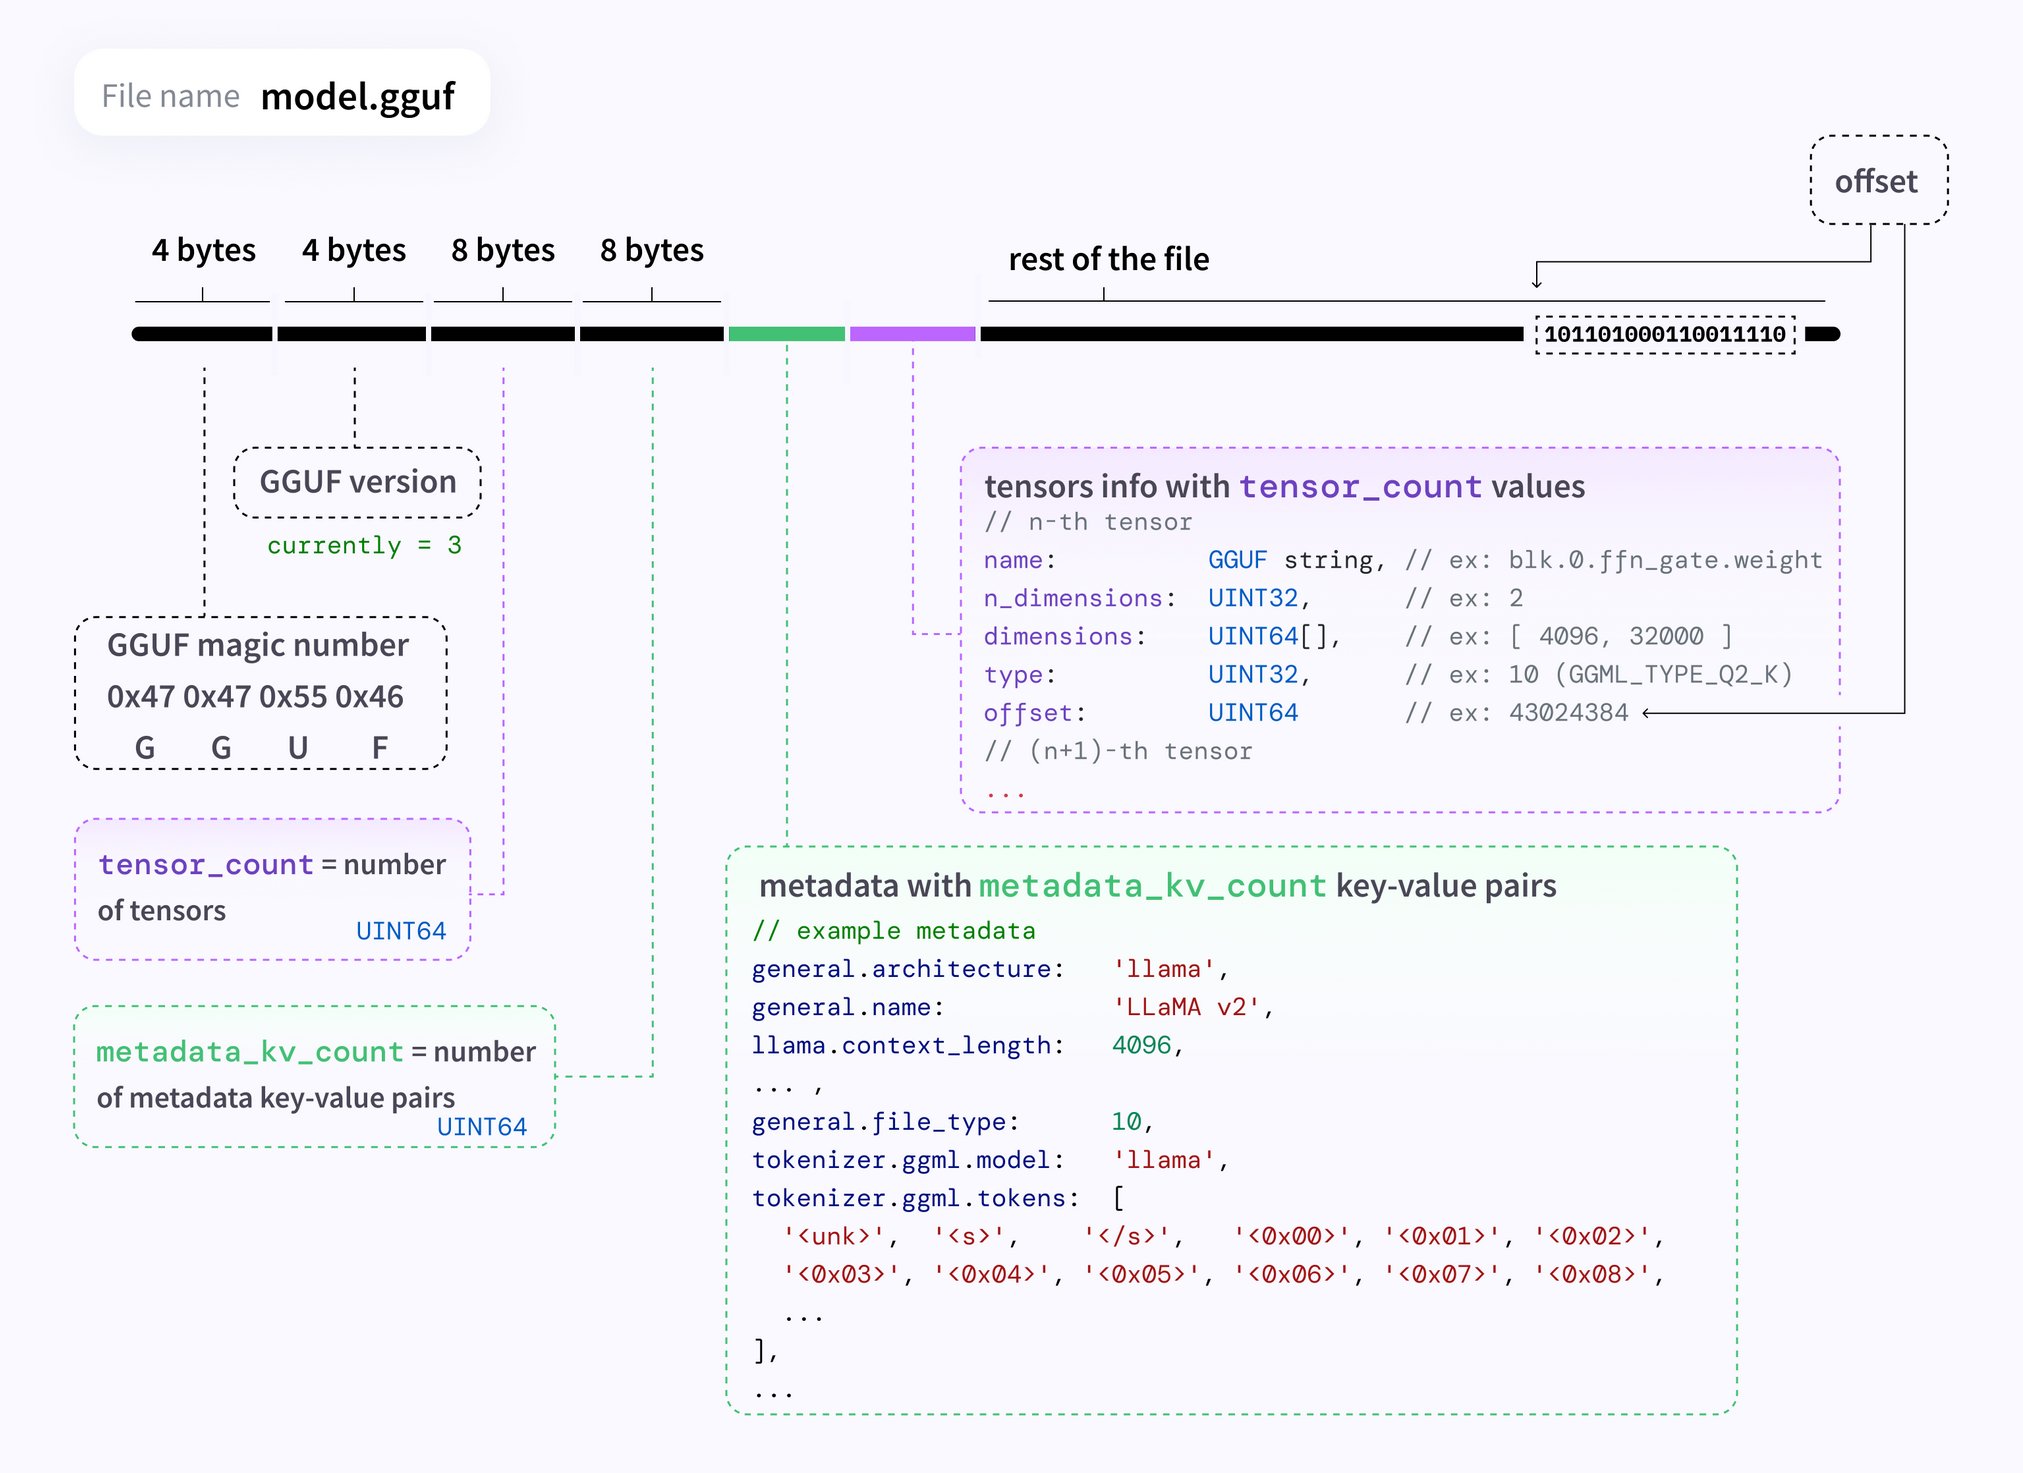
\includegraphics[width=\linewidth]{gguf}
			\caption{GGUF Format Breakdown}
			\label{fig:gguf}
		\end{center}
	\end{figure}
	
	
	\subsection{\gls{llm} Pruning}
	
	\subsection{\gls{llm} Benchmarking}
	
	\section{Working Theory}
	
	\section{Research Design}
	\subsection{Introduction}
	\subsection{Design}
	
	\section{Conclusion}
	
	\bibliography{proposal}
	
	\printglossary[title={Abbreviations}]
	
	\appendix
	\section{Appendix A}
\end{document}
